\documentclass[10pt]{article}
\usepackage[utf8]{inputenc}
\usepackage[OT1]{fontenc}
\usepackage{amsfonts, amsmath, amsthm, amssymb}
\usepackage{natbib}
\usepackage{graphicx}
\usepackage{listings}
\usepackage[margin=1in]{geometry}
\usepackage{xcolor}
\usepackage{bigints}
\usepackage{glossaries}
\usepackage{graphicx}
\graphicspath{ {./images/} }


\newcounter{countCode}
\lstnewenvironment{code} [1][caption=Ponme caption, label=default]{%
	\renewcommand*{\lstlistingname}{Listado} 
	\setcounter{lstlisting}{\value{countCode}} 
	\lstset{ %
	language=java,
	basicstyle=\ttfamily\footnotesize,       % the size of the fonts that are used for the code
	numbers=left,                   % where to put the line-numbers
	numberstyle=\sc,      % the size of the fonts that are used for the line-numbers
	stepnumber=1,                   % the step between two line-numbers. 
	numbersep=5pt,                 % how far the line-numbers are from the code
	numberstyle=\color{red!50!blue},
    	backgroundcolor=\color{lightgray!20},
	rulecolor=\color{blue},
	keywordstyle=\color{red}\bfseries,
	showspaces=false,               % show spaces adding particular underscores
	showstringspaces=false,         % underline spaces within strings
	showtabs=false,                 % show tabs within strings adding particular underscores
	frame=single,                   % adds a frame around the code
	framexleftmargin=0mm,
	numberblanklines=false,
	xleftmargin=5pt,
	breaklines=true,
	breakatwhitespace=true,
	breakautoindent=true,
	captionpos=t,
	texcl=true,
	tabsize=2,                      % sets default tabsize to 3 spaces
	extendedchars=true,
	inputencoding=utf8, 
	escapechar=\%,
	morekeywords={print, println, size, background, strokeWeight, fill, line, rect, ellipse, triangle, arc, save, PI, HALF_PI, QUARTER_PI, TAU, TWO_PI, width, height,},
	emph=[1]{print,println,}, emphstyle=[1]{\color{blue}}, % Mis palabras clave.
	emph=[2]{width,height,}, emphstyle=[2]{\bf\color{violet}}, % Mis palabras clave.
	emph=[3]{PI, HALF_PI, QUARTER_PI, TAU, TWO_PI}, emphstyle=[3]\color{orange!50!violet}, % Mis palabras clave.
	emph=[4]{line, rect, ellipse, triangle, arc,}, emphstyle=[4]\color{green!70!black}, % Mis palabras clave.
	%emph=[5]{size, background, strokeWeight, fill,}, emphstyle=[5]{\tt \color{red!30!blue}}, % Mis palabras clave.
	%emph={[2]sqrt,baset}, emphstyle={[2]\color{blue}}, % f(sqrt(2)), sqrt a nivel 2 se pondrá azul
	#1}}{\addtocounter{countCode}{1}}



\title{A Pot-Pourri of Probability \& Optimal Transport}
\author{Davi Sales Barreira}
\date{\today}
\begin{document}
\maketitle \tableofcontents 


\begin{abstract}
The main goal of these notes is to present an introduction to the transport inequalities,
which consist of methods of using Optimal Transport Theory to obtain concentration
inequalities in high-dimensional probability. Along the way, as new concepts are presented,
some side-lining will be done, with the aim to explore some of these new concepts, before
diving back in the proof of the inequalities.
\end{abstract}

\section*{Notation}
\begin{itemize}
	\item $P(\mathcal X)$ - S
	Most of the content regarding transportation inequality is from

\end{itemize}
\section{Introduction}
Given two probability distributions $\mu,\nu$, there are many situations
where one is interested in defining a way of measuring the
distance between them. The Wasserstein distance is a
metric that arises from the idea of optimal transport, and which has being
gaining attention in Statistics and Machine Learning. One prominent example is the so
called Wasserstein Generative Adversarial Network (WGAN), which uses this metric to evaluate
how well the model generated distribution approximates the "real" distribution of the
data. As will be shown shortly, the Wasserstein metric has several advantages compared to
other metrics.

There are several ways of defining distances between two
probability measures. Let's assume that $\nu, \mu$ are defined on 
$(\Omega, \mathcal F)$ and that $\nu \ll \lambda$,
$\mu \ll \lambda$ , for $\lambda$ representing the Lebesgue measure. Below
we present some example of distances:

\begin{align*} 
\text{Total Variation} &: \quad || \mu - \nu ||_{TV} =
\sup_{A \in \mathcal F} |\mu (A) - \nu(A)| = 
\frac{1}{2}\int_\Omega \left | \frac{d\mu}{d\lambda} - \frac{d\nu}{d\lambda} \right
|d\lambda \\
\\
\text{Hellinger} &: \quad \sqrt{\bigintss_\Omega \left(\sqrt{\frac{d\mu}{d\lambda}} -
\sqrt{\frac{d\nu}{d\lambda}} \right )^2d\lambda} \\
\\
L_2 &: \quad \int_\Omega \left(\frac{d\mu}{d\lambda} - \frac{d\nu}{d\lambda}\right)^2
d\lambda \\
% \text{Relative Entropy} &: \quad
% H(\nu \mid \mu) =
% \left\{
%   \begin{array}{@{}ll@{}}
%     \int_\mathcal X \log(\frac{d\nu}{d\mu})d\nu, & \text{if}\ \nu \ll\mu \\
%     +\infty, & \text{otherwise}
%   \end{array}\right.
%   \\
%   \\
\end{align*}

As pointed out by \citet{wassermanStatisicalMethods2018} in his lecture notes,
although such distances are useful, there are drawbacks:
\begin{itemize}
	\item If one distribution is discrete and the other is continuous,  they cannot
	be compared. If $X \sim U(0,1)$ and $Y$ is uniform on $\{0,1/N, 2/N,...,1\}$,
	although this distributions are very similar, their total variation is 1 (which is
	the maximum value). The Wasserstein distance is $1/N$, which is reasonable.
	\item These distances ignore the "geometry of the underlying space", while the
	Wasserstein distance preserves it, as shown in Figure~\ref{fig:distances}.
\end{itemize}
\begin{figure}[h]
	\centering
	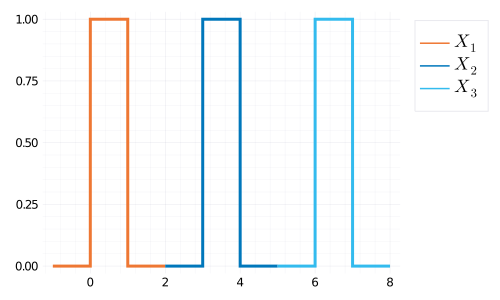
\includegraphics[width=10cm]{images/Distributions_Distances.png}
    \caption{Each pair has the same distance in $L_2$, Hellinger and TV. But using
    Wasserstein, $X_1$ is closer to $X_2$ than to $X_3$.}
    \label{fig:distances}
\end{figure}



% \begin{equation}
% \textbf{A} = \left[
% \begin{array}{cccc}
% a_{11} & a_{12} & \cdots & a_{1m} \\
% a_{21} & a_{22} & \cdots & a_{2m} \\
% \vdots & \vdots & \ddots & \vdots \\
% a_{n1} & a_{n2} & \cdots & a_{nm} \\
% \end{array}
% \right]
% \end{equation}

% \begin{itemize}
%  \item Cada uno de los números de que consta la matriz se denomina \textbf{elemento}. Un elemento se distingue de otro por la posición que ocupa, es decir, la fila y la columna a la que pertenece. Para ello se usa un doble subíndice donde el primero indica la fila y el segundo la columna a la que pertenece.
 
%  Una forma simplificada de representar una matriz es $A:= ((a_{ij}))$
%  \item El número de filas y columnas de una matriz se denomina \textbf{dimensión de una matriz}. A una matriz con n filas y m columnas se le denomina matriz n-por-m (escrito $n\times{m}$) donde n, m $\in{\mathbb{N}} - \{0\}$.
%  \item Si la matriz tiene el mismo número de filas que de columnas, y es $n$, se dice que es de \textbf{orden} $n$.
%  \item Dos matrices son \textbf{iguales} cuando tienen la misma dimensión y los elementos que ocupan el mismo lugar en ambas, son iguales.
%  \item El conjunto de las matrices de tamaño $n \times{m}$ se representa como $\mathcal{M}_{n\times {m}}(\mathbb{K})$ donde $\mathbb{K}$ es el campo al cual pertenecen las entradas. El tamaño de una matriz siempre se da con el número de filas primero y el número de columnas después.
%  \end {itemize}
 
% \section{Tipos de Matrices}

% \noindent\textbf{Matriz fila:} Una matriz fila está constituida por una sola fila.

% \[\begin{bmatrix}
% a_{11} & a_{12} & \cdots & a_{1m} \\
% \end{bmatrix}\]

% \noindent\textbf{Matriz columna:} La matriz columna tiene una sola columna.

% \[\begin{bmatrix}
% a_{11} \\
% a_{21} \\
% \vdots \\
% a_{n1} \\
% \end{bmatrix}\]

% \textbf{Matriz rectangular:} La matriz rectangular tiene distinto número de filas que de columnas, siendo su dimensión $n\times {m}$. (Ver expresión (1)).

% \textbf{Matriz traspuesta:} Dada una matriz $A$, se llama matriz traspuesta de A a la matriz que se obtiene cambiando ordenadamente las filas por las columnas y se denota por $A^t$.

% Si A = (($a_{ij}$)), entonces $A^t$ = (($a_{ji}$))

% Cumplen las siguiente propiedades:

% \begin{itemize}
% \item $(A^t)^t = A$.
% \item $(A + B)^t = A^t + B^t$.
% \item $(\alpha \cdot )^t = \alpha \cdot {A^t}$
% \item $(A\times B)^t = B^t\times A^t$.
% \end{itemize}
% Las operaciones con matrices se definen en el apartado 3. \\


% \textbf{Matriz nula:} En una matriz nula todos los elementos son ceros. $A = ((a_{ij})) = ((0))$ \\

% \textbf{Matriz cuadrada:} La matriz cuadrada tiene el mismo número de filas que de columnas.

% \begin{itemize}
% \item Los elementos de la forma $((a_{ii}))$ constituyen \textbf{la diagonal principal}.
% \item La \textbf{diagonal secundaria} la forman los elementos con $i + j = n + 1$, siendo $n$ el orden de la matriz.
% \item Existen los siguientes tipos de matrices cuadradas\footnote{Las operaciones con matrices se definen en el apartado 3.}

% \textit{Matriz triangular superior:} En una matriz triangular superior los elementos situados por debajo de la diagonal principal son ceros.

% $$\textbf{A=}\begin{bmatrix}
% a_{11} & a_{12} & \cdots & a_{1m} \\
% 0 & a_{22} & \cdots & a_{2m} \\
% \vdots & \vdots & \ddots & \vdots \\
% 0 & 0 & \cdots & a_{nm}
% \end{bmatrix}
% $$

% \textit{Matriz triangular inferior:} En una matriz triangular inferior los elementos situados por encima de la diagonal principal son ceros.

% $$\textbf{A=}\begin{bmatrix}
% a_{11} & 0 & \cdots & 0 \\
% a_{21} & a_{22} & \cdots & 0 \\
% \vdots & \vdots & \ddots & \vdots \\
% a_{n1} & a_{n2} & \cdots & a_{nm}
% \end{bmatrix}
% $$

% \textit{Matriz diagonal:} En una matriz diagonal todos los elementos que no están situados en la diagonal principal son nulos.

% $$\textbf{A=}\begin{bmatrix}
% a_{11} & 0 & \cdots & 0 \\
% 0 & a_{22}  & \cdots & 0 \\
% \vdots & \vdots & \ddots & \vdots \\
% 0 & 0 & \cdots & a_{nm}
% \end{bmatrix}
% $$

% \textit{Matriz escalar:} Una matriz  escalar es una matriz diagonal en la que los elementos de la diagonal principal son iguales.

% \textit{Matriz identidad o unidad:} Una matriz  identidad es una matriz diagonal en la que los elementos de la diagonal principal son iguales a 1.

% \textit{Matriz regular:} Una matriz  regular es una matriz cuadrada que tiene inversa.

% \textit{Matriz singular:} Una matriz  singular no tiene matriz inversa.

% \textit{Matriz indempotente:} Una matriz, $A$, es indempotente si: $A^2 = A$.

% \textit{Matriz involutiva:} Una matriz, $A$, es involutiva si: $A^2 = I$.

% \textit{Matriz simétrica:} Una matriz simétrica es una matriz cuadrada que verifica: $A = A^t$.
% \textit{Matriz antisimétrica o hemisimétrica:} Una matriz antisimétrica o hermisimétrica es una matriz cuadrada que verifica $A = -A^t$.

% \textit{Matriz ortogonal:} Una matriz es ortogonal si verifica que: $A\times {A^t} = I$

% \end{itemize}

% \section{Operaciones con Matrices}
% Las operaciones que se pueden hacer con matrices provienen de sus aplicaciones, sobre todo de las aplicaciones en álgebra lineal. De ese modo las operaciones, o su forma muy particular de ser implementadas, no son únicas.

% \subsection{Suma o adición}

% \noindent \textbf{Definición}

% Se define la operación de suma o adición de matrices como una operación binaria
% \section*{References}
% \addcontentsline{toc}{section}{References}
  \bibliography{probability_ot}
  \bibliographystyle{plainnat}
  % \bibliographystyle{plainnat}
  % \bibliographystyle{plain}
  % \bibliographystyle{abbrv}
\end{document}

